\documentclass[a4paper,12pt]{report}
\usepackage{float}
\usepackage{setspace}
\usepackage[utf8]{inputenc}
\usepackage[T1]{fontenc}
\usepackage[english]{babel}
\usepackage{xcolor,graphicx, tikz}
\usepackage[top=0.3in,bottom=0in,right=1in,left=1in]{geometry}
\usepackage{background}
\usepackage{hyperref, url, float}
\usepackage{titlesec}
\usepackage{listings}
\usepackage{color}
\usepackage{minted}
\usepackage{tcolorbox}
\usepackage{xcolor}
\usepackage{xurl}

\hypersetup{
    colorlinks=true,
    linkcolor=black,
    urlcolor=blue,
    pdfborder={0 0 0}, % Set border color to black
}
\usepackage{fix-cm}
\usepackage[bf]{caption}
\usepackage{subcaption}
\usepackage{amssymb}
\usepackage[fleqn]{amsmath,mathtools}
\usepackage{fancyhdr}
\usepackage[Lenny]{fncychap}
\usepackage{hyperref}
\ChTitleVar{\Huge\bfseries}
\ChNameVar{\large\bfseries}
\ChNumVar{\fontsize{60}{62}\bfseries}

%\setcounter{tocdepth}{4}

\setlength{\parskip}{0.2cm} % Set vertical space between paragraphs to 0.2cm

\titleformat{\section}{\normalfont\Large\bfseries}{\thesection}{1em}{}
\titlespacing*{\section}{0pt}{3pt}{2pt}
% Define background image
\usepackage{array}
\newcolumntype{P}[1]{>{\centering\arraybackslash}p{#1}}
\definecolor{codegreen}{rgb}{0,0.6,0}
\definecolor{codegray}{rgb}{0.5,0.5,0.5}
\definecolor{codepurple}{rgb}{0.58,0,0.82}
\definecolor{backcolour}{rgb}{0.95,0.95,0.92}
\lstdefinestyle{Arduino}{
    backgroundcolor=\color{backcolour},
    commentstyle=\color{codegreen},
    keywordstyle=\color{magenta},
    numberstyle=\tiny\color{codegray},
    stringstyle=\color{codepurple},
    basicstyle=\footnotesize,
    breakatwhitespace=false,
    breaklines=true,
    captionpos=b,
    keepspaces=true,
    numbers=left,
    numbersep=5pt,
    showspaces=false,
    showstringspaces=false,
    showtabs=false,
    tabsize=2
}
\lstset{style=Arduino}
\begin{document}
\begin{titlepage}
    \backgroundsetup{
    contents={
\includegraphics[width=1.5cm,height=\paperheight]{Pics/rightPadUMI.jpeg}}, 
    angle=0,
    position=current page.east,
    vshift=0pt,
    hshift=0pt,
    opacity=1,
    scale=1
    }
    \begin{center}
        
        \begin{minipage}{13cm}
        	\begin{center}
        		
\includegraphics[width=8.5cm,height=2.5cm]{Pics/LOGO_FS2_rapport.jpg}
        	\end{center}
        \end{minipage}\hfill
        
        
        %\includegraphics[width=0.6\textwidth]{logo-isae-supaero}\\[1cm]
        \textsc{\Large }\\[1cm]
        {{\fontsize{18pt}{18pt}\selectfont\textbf{Department of IT}}}\\[0.6cm]
        {\large \textbf{ Licence Program :}}\\[0.6cm]
        {\large \textbf{Mathematical Sciences and Computer Science (SMI)}}\\[2cm]
        
        { {\fontsize{26pt}{26pt}\selectfont\textbf{End-of-studies project}}\\[1.5cm] }
        \begin{flushleft}
             {\large \bfseries On the topic:}
        \end{flushleft}
       
        % Title
        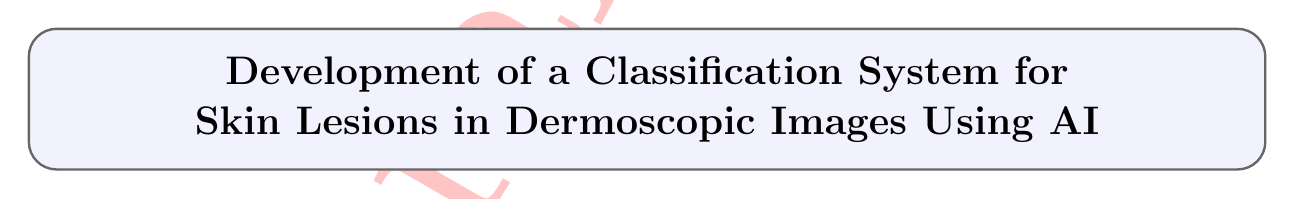
\begin{tikzpicture}
            \node[
                draw=black!60,
                line width=0.3mm,
                fill=blue!5,
                rounded corners=10pt,
                inner sep=10pt,
                align=center,
                text width=15cm,
                font=\Large\bfseries\color{black!70!black}
            ] 
            {Development of a Classification System for Skin Lesions in Dermoscopic Images Using AI};
        \end{tikzpicture}

        \noindent
        \begin{flushleft}
              \bf{Presented by :} \hspace{1.1cm} \textsc
            ~EL AMRAOUI \textbf{Khalil} \hspace{0.25cm} \&  \hspace{0.25cm} \textsc~TARIQ \textbf{Mohammed} 

        \end{flushleft}
        \begin{flushleft}
              \textbf{Supervised by :} \hspace{1cm} \textbf{Pr. \textsc{EL ANSARI } ~Mohamed} \hspace{2cm}
            \end{flushleft}

    \begin{flushleft}
         {\large \textit{Defended on Friday, 21st of June 2025, before the jury : }}\\[0.5cm]
    \end{flushleft}

%     \begin{tabular}{lll}
%         \bf \textbf{Pr. ~Abdelbaki \textsc{EL BELRHITI EL ALAOUI}}&  :&\bf \large Professeur à la FSM
%         \\[0.1cm]
%         \bf \textbf{Pr. ~Abdeslam \textsc{ELFERGOUGUI}}&  :&\bf \large Professeur à la FSM
%         \\[0.1cm]
%         \bf \textbf{Pr. ~El Mehdi \textsc{ISMAILI ALAOUI} }&  :&\bf \large Professeur à la FSM
%         \vspace{1cm}
%    \end{tabular}

    \bf \large{Academic Year 2024/2025 } \\[3.2cm]

        \begin{minipage}{17cm}
    	\begin{center}
    		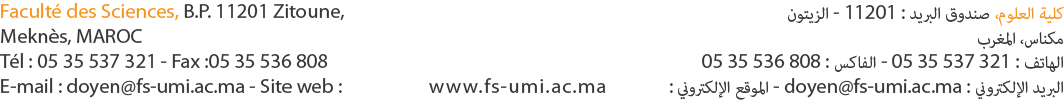
\includegraphics[width=17cm,height=2cm]{Pics/FooterUMI.png}
    	\end{center}
    \end{minipage}

    \end{center}
\end{titlepage}

\backgroundsetup{contents={}, }
\newgeometry{top=0.6in,bottom=0.6in,right=1in,left=1in}
\newpage
\begin{spacing}{1.5}
%-----------------------------------document begining-----------------------------------%
     \begin{center}
         \textbf{\huge Aknowledgements}
     \end{center}

    We would like to express our deepest gratitude to everyone who contributed to the successful completion of this project.

    First and foremost, we extend our sincere thanks to our supervisor, \textbf{Pr. ~Mohamed \textsc{El Ansari}}, for his unwavering support, guidance, and insightful feedback throughout the duration of this project. His expertise, patience, and encouragement have been instrumental in shaping both the direction and quality of this research, and for that, we are truly grateful.

    We would also like to extend our sincere appreciation to the distinguished members of the jury, who will dedicate their time and effort to evaluating this report. Their critical insights and feedback will undoubtedly enhance the quality of this work.

    Our  heartfelt thanks go to \textbf{Moulay Ismail University}, the \textbf{Faculty of Sciences}, and all the professors of the \textbf{Licence Program in SMI: Mathematical Sciences and Computer Science}. Their collective efforts in providing knowledge, resources, and academic guidance have been crucial in helping us achieve our academic goals throughout our undergraduate studies.

    Finally, our deepest gratitude is reserved for our family and friends, whose unwavering support and encouragement have been our greatest source of strength. Their belief in us has been invaluable in overcoming the challenges faced during our undergraduate studies. We truly could not have reached this point without them.

\newpage
\begin{center}
    \textbf{\huge Abstract}
\end{center}

    In the field of dermatological imaging, the accurate detection and classification of skin lesions is a critical task that significantly impacts early diagnosis and treatment planning for skin cancer. This report presents a comprehensive exploration of deep learning techniques, specifically focusing on the application of YOLOv8 framework for skin lesion detection and classification using dermoscopic images. By leveraging the real-time processing capabilities of YOLO architecture, coupled with advanced mosaic augmentation and class-balancing techniques, this work achieves high levels of accuracy in detecting and classifying melanoma, basal cell carcinoma (BCC), squamous cell carcinoma (SCC), and benign nevus.

    The proposed model was assessed using standard evaluation metrics including accuracy, precision, recall, and F1-score, demonstrating exceptional performance with 93.35\% overall accuracy and class-specific F1-scores up to 0.97 for melanoma detection. Implemented as a standalone desktop application using Tkinter, it provides dermatologists with an intuitive graphical interface for local image analysis without requiring internet connectivity or cloud dependencies. This offline capability ensures patient data privacy compliance while enabling efficient lesion classification in resource-limited settings.

    This research contributes to the growing field of AI-assisted dermatology while highlighting YOLO's potential to revolutionize skin cancer diagnostics through efficient, scalable solutions. Future directions for this work include the expansion of the dataset, enhancing the Tkinter GUI for clinical use, and the integration of skin lesion segmentation capabilities to further improve diagnostic accuracy.


    \newpage
\begin{center}
    \textbf{\huge Résumé}
\end{center}

    Dans le domaine de l'imagerie dermatologique, la détection et la classification précises des lésions cutanées constituent une tâche cruciale ayant un impact significatif sur le diagnostic précoce et la planification thérapeutique du cancer de la peau. Ce rapport présente une exploration approfondie des techniques d'apprentissage profond, en se concentrant spécifiquement sur l'application du framework YOLOv8 pour la détection et la classification des lésions cutanées à l'aide d'images dermoscopiques. En tirant parti des capacités de traitement en temps réel de l'architecture YOLO, combinées à des techniques avancées d'augmentation de données (mosaic augmentation) et d'équilibrage des classes, ce travail atteint un haut niveau de précision dans la détection et la classification du mélanome, du carcinome basocellulaire (CBC), du carcinome épidermoïde (CE) et du nævus bénin.

    Le modèle proposé a été évalué à l'aide de métriques standards incluant l'exactitude, la précision, le rappel et le F1-score, démontrant des performances exceptionnelles avec une exactitude globale de 93,35\% et des F1-scores atteignant 0,97 pour la détection du mélanome. Implémenté sous forme d'application desktop autonome utilisant Tkinter, il fournit aux dermatologues une interface graphique intuitive pour l'analyse locale d'images sans nécessiter de connectivité internet ni dépendances cloud. Cette capacité hors-ligne garantit la conformité aux réglementations sur la confidentialité des données médicales tout en permettant une classification efficace des lésions dans des environnements à ressources limitées.

    Cette recherche contribue au domaine croissant de la dermatologie assistée par l'IA, tout en soulignant le potentiel de YOLO à révolutionner le diagnostic du cancer de la peau grâce à des solutions efficaces et évolutives. Les perspectives futures de ce travail incluent l'élargissement du jeu de données, l'amélioration de l'interface Tkinter pour un usage clinique et l'intégration de fonctionnalités de segmentation des lésions cutanées afin d'améliorer encore la précision diagnostique.
    
\tableofcontents
\listoffigures
\listoftables


\chapter{General Introduction}
    \section{Context}
    Skin cancer is one of the most prevalent forms of cancer worldwide, accounting for a significant number of cancer diagnoses annually. Among its various types, melanoma poses the highest threat due to its aggressive nature and high mortality rate if not detected early. Early and accurate diagnosis of skin lesions, particularly melanoma, is vital to improving patient outcomes and survival rates. Dermoscopic imaging, a non-invasive technique that magnifies skin structures, has become a cornerstone in dermatology for identifying and classifying skin lesions. However, the interpretation of dermoscopic images is a challenging task, requiring extensive training and expertise, and is often subject to human error \cite{intro1}\cite{intro2}.
    % \addcontentsline{toc}{chapter}{Introduction générale}
    
    The emergence of artificial intelligence (AI) has revolutionized various domains, including healthcare. AI-powered systems have shown remarkable potential in analyzing medical images, aiding clinicians in diagnosing diseases more accurately and efficiently. Leveraging AI for skin lesion classification offers a promising avenue to bridge the gap in expertise and resources, particularly in underserved regions with limited access to dermatologists. By automating the process of analyzing dermoscopic images, AI systems can assist in early detection and treatment, ultimately saving lives\cite{intro3}\cite{intro4}.
    \newpage

    \section{Problem Statement}
    Despite advancements in dermoscopic imaging and AI, developing a reliable classification system for skin lesions remains a challenging endeavor. Medical image classification poses unique difficulties, such as:
    \begin{enumerate}
        \item Variability in lesion appearance due to differences in color, texture, and shape.
        \item The imbalance in datasets, where certain lesion types are underrepresented, leading to biased models.
        \item The need for high accuracy and specificity to minimize false positives and negatives, as misdiagnoses can have severe consequences.
        \item Integration challenges requiring interpretability and trustworthiness.
    \end{enumerate}
    These challenges underscore the need for robust AI systems capable of handling dermoscopic image nuances\cite{intro5}\cite{intro6}.

    \section{Objectives}
    The primary objectives of this project are:
    \begin{enumerate}
        \item \textbf{Develop a YOLOv8-Based Classification System} To design and implement a classification system for dermoscopic images using YOLOv8, leveraging its state-of-the-art performance to identify and categorize various skin lesion types effectively \cite{intro7}\cite{intro8}.
        \item \textbf{Optimize Model Selection and Performance} To evaluate and compare the performance of YOLOv8 model variants (n, m, x) based on metrics such as accuracy, specificity, and generalizability, identifying the optimal variant for the classification task \cite{intro9}.
        \item \textbf{Address Dataset Challenges} To mitigate challenges such as class imbalance and variability in lesion appearance by applying advanced preprocessing techniques, data augmentation, and model fine-tuning for enhanced classification results \cite{intro8}\cite{intro10}.
        \item \textbf{Document Challenges and Recommendations} To document the development process, highlight the challenges encountered, and provide actionable recommendations for improving YOLOv8-based classification systems in medical imaging \cite{intro7}\cite{intro9}.
    \end{enumerate}

    \section{Structure of the Report}
    This report is organized as follows:

    \begin{itemize}
        \item \textbf{Chapter 1: General Introduction} \\
        Outlines the clinical and technical context of skin lesion classification. Defines the problem statement, objectives, and significance of the project.

        \item \textbf{Chapter 2: Deep Learning Overview} \\
        Provides a comprehensive overview of deep learning concepts, focusing on computer vision applications. Discusses classification techniques and their relevance to medical imaging.

        \item \textbf{Chapter 3: State of the Art} \\
        modify !!!!

        \item \textbf{Chapter 4: Proposed Solution: YOLOv8} \\
        Describes the YOLOv8 architecture and its advantages for skin lesion classification. Details the dataset used, preprocessing steps, and model training process.

        \item \textbf{Chapter 5: Discussion} \\
        Analyzes the results of the YOLOv8 model, comparing its performance with existing methods. Discusses the implications of findings for clinical practice and future research directions.

        \item \textbf{Chapter 6: Conclusion} \\
        Summarizes the key findings of the project, reflecting on the objectives achieved and the challenges encountered. Provides recommendations for future work in skin lesion classification using AI.

    \end{itemize}



\chapter{Deep Learning Overview}
    \section{Definition}
    Deep learning (DL) is a subfield of machine learning that employs artificial neural networks with multiple layers (deep architectures) to model complex patterns in data. Unlike traditional machine learning, which relies on manual feature engineering, DL automates feature extraction through hierarchical learning, enabling it to excel in tasks like image recognition, natural language processing, and decision-making \cite{dl}. Its significance lies in its ability to process unstructured data (e.g., images, text) at scale, driving breakthroughs in autonomous systems, healthcare diagnostics, and personalized recommendations \cite{dl2}.

    \begin{minipage}[lH]{0.8\textwidth}
        \centering
        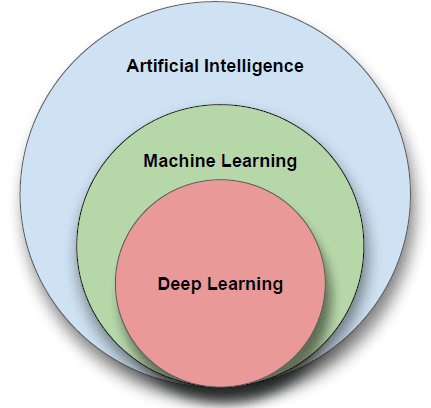
\includegraphics[width=10cm, height=10cm]{Pics/deepLearning.png}
        \captionof{figure}{Deep Learning Overview}
    \end{minipage} 
    \hspace{1cm}
    \begin{minipage}[rH]{0.1\textwidth}
        \cite{dlImg}    
    \end{minipage}
    
    \vspace{0.5cm}

    \section{Computer Vision in Deep Learning}
    Computer vision (CV) leverages DL to interpret visual data. Techniques such as Convolutional Neural Networks (CNNs) dominate this domain, using convolutional layers to extract spatial hierarchies of features from images \cite{dl3}. Applications include:
    \begin{itemize}
        \item \textbf{Image Classification:} Identifying objects in images (e.g., distinguishing benign vs. malignant skin lesions).
        \item \textbf{Object Detection:} Locating and classifying multiple objects within an image (e.g., tumors in medical scans).
        \item \textbf{Semantic Segmentation:} Pixel-level labeling for precise delineation (e.g., tumor boundaries)~\cite{dl4}.

    These methods underpin advancements in medical imaging, enabling automated analysis of X-rays, MRIs, and dermatology images~\cite{dl5}.
    \end{itemize}
    \hspace{3cm}
    \begin{center}
        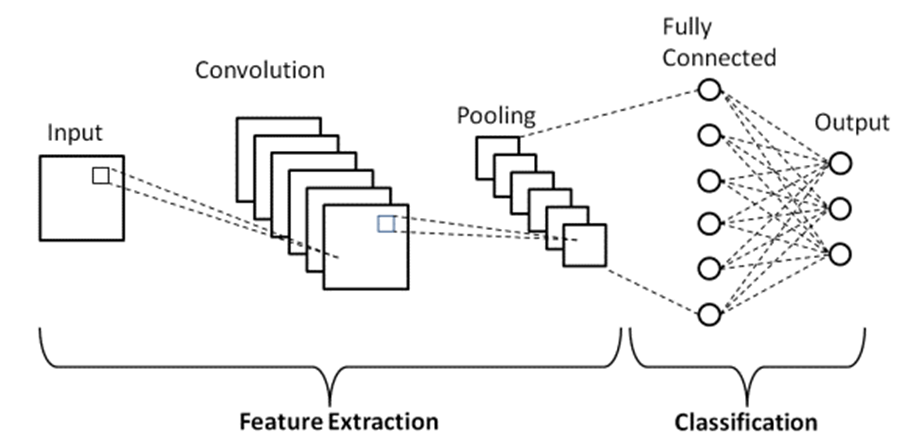
\includegraphics[width=14cm, height=6cm]{Pics/cnn1.png}
        \captionof{figure}{Convolutional Neural Network for Computer Vision}   
    \end{center}
    \hspace{1cm}
    \begin{minipage}[rH]{0.1\textwidth}
        \cite{cnnImg}    
    \end{minipage}

    \section{Classification}
    Classification involves categorizing input data into predefined classes. In DL, this is typically achieved using softmax activation in the final layer of a neural network. For medical projects like skin cancer diagnosis, classification tasks are critical for:
    \begin{itemize}
        \item \textbf{Binary Classification:} Differentiating malignant vs. benign lesions.
        \item \textbf{Multi-Class Classification:} Identifying specific cancer subtypes (e.g., melanoma, basal cell carcinoma)~\cite{dl6}.
    \end{itemize}
      Performance metrics such as accuracy, sensitivity, and specificity are used to evaluate model reliability~\cite{dl7}.
    
    \section{Deep Learning in Medicine}
    DL has revolutionized healthcare with applications such as:

    \begin{itemize}
        \item \textbf{Diagnostic Imaging:} Google’s DL model achieved 94\% accuracy in detecting diabetic retinopathy from retinal scans~\cite{dl8}.
        \item \textbf{Drug Discovery:} DeepMind’s AlphaFold predicts protein structures, accelerating drug development~\cite{dl9}.
        \item \textbf{Pathology:} Algorithms like PathAI assist pathologists in identifying cancer metastases in histopathology slides~\cite{dl10}.
    \end{itemize}
    Challenges include data privacy, model interpretability, and integration into clinical workflows~\cite{dl11}.
    
    \section{Types of Diseases Addressed}
    This project focuses on skin cancer, a critical global health concern. Key types include:
    
    \begin{itemize}
        \item \textbf{Melanoma:} The most aggressive form of skin cancer, responsible for the majority of skin cancer-related fatalities due to its metastatic potential~\cite{dl12}.
        \item \textbf{Basal Cell Carcinoma (BCC):} The most common skin cancer, characterized by slow growth and rare metastasis.
        \item \textbf{Squamous Cell Carcinoma (SCC):} A faster-growing cancer with higher metastatic risk compared to BCC~\cite{dl13}.
        \item \textbf{Nevus (Benign Melanocytic Lesions):} Common non-cancerous moles that require differentiation from melanoma to avoid misdiagnosis~\cite{dl14}.
    \end{itemize}
    The dataset includes dermoscopic images of these lesions, emphasizing the critical need for accurate classification to reduce unnecessary biopsies for benign cases like nevus while ensuring early detection of malignancies~\cite{dl15}.


\chapter{}

\begin{thebibliography}{99}

\addcontentsline{toc}{chapter}{Bibliographie}


\bibitem[Sung21]{intro1}
 \emph{Sung, H. et al. (2021). Global Cancer Statistics 2020. CA: A Cancer Journal for Clinicians.}

\bibitem[Kittler16]{intro2}
 \emph{Kittler, H. et al. (2016). Standardization of Terminology in Dermoscopy. Journal of the American Academy of Dermatology.}

\bibitem[Esteva17]{intro3}
 \emph{Esteva, A. et al. (2017). Dermatologist-Level Classification of Skin Cancer with Deep Neural Networks. Nature.}

\bibitem[Brinker19]{intro4}
 \emph{Brinker, T. J. et al. (2019). Deep Learning Outperformed 136 of 157 Dermatologists. European Journal of Cancer.}

\bibitem[Tschandl18]{intro5}
 \emph{Tschandl, P. et al. (2018). The HAM10000 Dataset. Scientific Data.}

\bibitem[Haenssle18]{intro6}
 \emph{Haenssle, H. A. et al. (2018). Man Against Machine. Journal of the European Academy of Dermatology and Venereology.}

\bibitem[LeCun15]{intro7}
 \emph{LeCun, Y., Bengio, Y., and Hinton, G. (2015). Deep learning. Nature, 521(7553), 436-444.}

\bibitem[Esteva17b]{intro8}
 \emph{Esteva, A., Kuprel, B., Novoa, R. A., et al. (2017). Dermatologist-level classification of skin cancer with deep neural networks. Nature, 542(7639), 115-118.}

\bibitem[Howard20]{intro9}
 \emph{Howard, J., and Gugger, S. (2020). Deep Learning for Coders with fastai and PyTorch. O'Reilly Media.}

\bibitem[ISIC]{intro10}
 \emph{ISIC Archive: International Skin Imaging Collaboration. Retrieved from \url{https://www.isic-archive.com}}



\bibitem[Goodfellow16]{dl}
 \emph{Goodfellow, I., Bengio, Y., and Courville, A. (2016). Deep Learning. MIT Press.}

\bibitem[LeCun15]{dl2}
 \emph{LeCun, Y., Bengio, Y., and Hinton, G. (2015). Deep Learning. Nature, 521(7553), 436–444.}

\bibitem[Ronneberger15]{dl3}
 \emph{Ronneberger, O., Fischer, P., and Brox, T. (2015). U-Net: Convolutional Networks for Biomedical Image Segmentation. MICCAI.}

\bibitem[Ronneberger15b]{dl4}
 \emph{Ronneberger, O., Fischer, P., and Brox, T. (2015). U-Net: Convolutional Networks for Biomedical Image Segmentation. MICCAI.}

\bibitem[Esteva17b]{dl5}
 \emph{Esteva, A., et al. (2017). Dermatologist-Level Classification of Skin Cancer with Deep Neural Networks. Nature, 542(7639), 115–118.}

\bibitem[He16]{dl6}
 \emph{He, K., et al. (2016). Deep Residual Learning for Image Recognition. CVPR.}

\bibitem[Litjens17]{dl7}
 \emph{Litjens, G., et al. (2017). A Survey on Deep Learning in Medical Image Analysis. Medical Image Analysis, 42, 60–88.}

\bibitem[Gulshan16]{dl8}
 \emph{Gulshan, V., et al. (2016). Development and Validation of a Deep Learning Algorithm for Detection of Diabetic Retinopathy in Retinal Fundus Photographs. JAMA, 316(22), 2402–2410.}

\bibitem[Jumper21]{dl9}
 \emph{Jumper, J., et al. (2021). Highly Accurate Protein Structure Prediction with AlphaFold. Nature, 596(7873), 583–589.}

\bibitem[Bera19]{dl10}
 \emph{Bera, K., et al. (2019). Artificial Intelligence in Digital Pathology. Nature Reviews Cancer, 19(12), 703–715.}

\bibitem[Topol19]{dl11}
 \emph{Topol, E. J. (2019). High-Performance Medicine: The Convergence of Human and Artificial Intelligence. Nature Medicine, 25(1), 44–56.}

\bibitem[ACS23]{dl12}
 \emph{American Cancer Society. (2023). Skin Cancer Facts and Statistics.}

\bibitem[Rogers15]{dl13}
 \emph{Rogers, H. W., et al. (2015). Incidence Estimate of Nonmelanoma Skin Cancer in the U.S., 2006. Archives of Dermatology, 146(3), 283–287.}

\bibitem[Tschandl18b]{dl14}
 \emph{Tschandl, P., et al. (2018). The HAM10000 Dataset: A Large Collection of Multi-Source Dermatoscopic Images of Common Pigmented Skin Lesions. Scientific Data, 5, 180161.}

\bibitem[Marchetti18]{dl15}
 \emph{Marchetti, M. A., et al. (2018). Results of the 2016 International Skin Imaging Collaboration International Symposium on Biomedical Imaging Challenge: Comparison of the Accuracy of Computer Algorithms to Dermatologists for the Diagnosis of Melanoma from Dermoscopic Images. Journal of the American Academy of Dermatology, 78(2), 270–277.}




\bibitem[DL]{dlImg}
 \emph{\url{https://levelup.gitconnected.com/introduction-to-neural-networks-and-deep-learning-3f44e3e50196}}

 \bibitem[CNN]{cnnImg}
    \emph{\url{https://www.nomidl.com/computer-vision/how-to-build-a-convolutional-neural-network-for-computer-vision/}}


\end{thebibliography}

\end{spacing}
\end{document}